\begin{figure}
  \centering

  \small

  \newcommand{\w}[1]{\textcolor{white}{#1}}
  \def\svgwidth{0.9\textwidth}

  % INKSCAPE
%% Creator: Inkscape inkscape 0.91, www.inkscape.org
%% PDF/EPS/PS + LaTeX output extension by Johan Engelen, 2010
%% Accompanies image file 'genmod.eps' (pdf, eps, ps)
%%
%% To include the image in your LaTeX document, write
%%   \input{<filename>.pdf_tex}
%%  instead of
%%   \includegraphics{<filename>.pdf}
%% To scale the image, write
%%   \def\svgwidth{<desired width>}
%%   \input{<filename>.pdf_tex}
%%  instead of
%%   \includegraphics[width=<desired width>]{<filename>.pdf}
%%
%% Images with a different path to the parent latex file can
%% be accessed with the `import' package (which may need to be
%% installed) using
%%   \usepackage{import}
%% in the preamble, and then including the image with
%%   \import{<path to file>}{<filename>.pdf_tex}
%% Alternatively, one can specify
%%   \graphicspath{{<path to file>/}}
%% 
%% For more information, please see info/svg-inkscape on CTAN:
%%   http://tug.ctan.org/tex-archive/info/svg-inkscape
%%
\begingroup%
  \makeatletter%
  \providecommand\color[2][]{%
    \errmessage{(Inkscape) Color is used for the text in Inkscape, but the package 'color.sty' is not loaded}%
    \renewcommand\color[2][]{}%
  }%
  \providecommand\transparent[1]{%
    \errmessage{(Inkscape) Transparency is used (non-zero) for the text in Inkscape, but the package 'transparent.sty' is not loaded}%
    \renewcommand\transparent[1]{}%
  }%
  \providecommand\rotatebox[2]{#2}%
  \ifx\svgwidth\undefined%
    \setlength{\unitlength}{560.96247387bp}%
    \ifx\svgscale\undefined%
      \relax%
    \else%
      \setlength{\unitlength}{\unitlength * \real{\svgscale}}%
    \fi%
  \else%
    \setlength{\unitlength}{\svgwidth}%
  \fi%
  \global\let\svgwidth\undefined%
  \global\let\svgscale\undefined%
  \makeatother%
  \begin{picture}(1,0.66882146)%
    \put(0,0){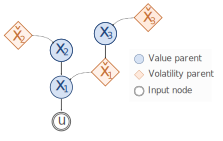
\includegraphics[width=\unitlength]{genmod.eps}}%
    \put(0.12848838,0.54400701){\color[rgb]{0,0,0}\makebox(0,0)[b]{\smash{$\check{x}_3$}}}%
    \put(0.34190334,0.54400701){\color[rgb]{0,0,0}\makebox(0,0)[b]{\smash{$x_3$}}}%
    \put(0.84380736,0.54400701){\color[rgb]{0,0,0}\makebox(0,0)[b]{\smash{$x_2$}}}%
    \put(0.62765594,0.54400701){\color[rgb]{0,0,0}\makebox(0,0)[b]{\smash{$\check{x}_2$}}}%
    \put(0.34190334,0.30869715){\color[rgb]{0,0,0}\makebox(0,0)[b]{\smash{$\check{x}_1$}}}%
    \put(0.84380736,0.30869715){\color[rgb]{0,0,0}\makebox(0,0)[b]{\smash{$x_1$}}}%
    \put(0.84380736,0.08572553){\color[rgb]{0,0,0}\makebox(0,0)[b]{\smash{$u$}}}%
  \end{picture}%
\endgroup%

  \caption{An example of a generative model of sensory inputs with six hidden states. Volatility coupling is depicted with dashed lines, value coupling with straight lines.}
  \label{\figlabel}
\end{figure}
